
% Default to the notebook output style

    


% Inherit from the specified cell style.




    
\documentclass[11pt]{article}

    
    
    \usepackage[T1]{fontenc}
    % Nicer default font (+ math font) than Computer Modern for most use cases
    \usepackage{mathpazo}

    % Basic figure setup, for now with no caption control since it's done
    % automatically by Pandoc (which extracts ![](path) syntax from Markdown).
    \usepackage{graphicx}
    % We will generate all images so they have a width \maxwidth. This means
    % that they will get their normal width if they fit onto the page, but
    % are scaled down if they would overflow the margins.
    \makeatletter
    \def\maxwidth{\ifdim\Gin@nat@width>\linewidth\linewidth
    \else\Gin@nat@width\fi}
    \makeatother
    \let\Oldincludegraphics\includegraphics
    % Set max figure width to be 80% of text width, for now hardcoded.
    \renewcommand{\includegraphics}[1]{\Oldincludegraphics[width=.8\maxwidth]{#1}}
    % Ensure that by default, figures have no caption (until we provide a
    % proper Figure object with a Caption API and a way to capture that
    % in the conversion process - todo).
    \usepackage{caption}
    \DeclareCaptionLabelFormat{nolabel}{}
    \captionsetup{labelformat=nolabel}

    \usepackage{adjustbox} % Used to constrain images to a maximum size 
    \usepackage{xcolor} % Allow colors to be defined
    \usepackage{enumerate} % Needed for markdown enumerations to work
    \usepackage{geometry} % Used to adjust the document margins
    \usepackage{amsmath} % Equations
    \usepackage{amssymb} % Equations
    \usepackage{textcomp} % defines textquotesingle
    % Hack from http://tex.stackexchange.com/a/47451/13684:
    \AtBeginDocument{%
        \def\PYZsq{\textquotesingle}% Upright quotes in Pygmentized code
    }
    \usepackage{upquote} % Upright quotes for verbatim code
    \usepackage{eurosym} % defines \euro
    \usepackage[mathletters]{ucs} % Extended unicode (utf-8) support
    \usepackage[utf8x]{inputenc} % Allow utf-8 characters in the tex document
    \usepackage{fancyvrb} % verbatim replacement that allows latex
    \usepackage{grffile} % extends the file name processing of package graphics 
                         % to support a larger range 
    % The hyperref package gives us a pdf with properly built
    % internal navigation ('pdf bookmarks' for the table of contents,
    % internal cross-reference links, web links for URLs, etc.)
    \usepackage{hyperref}
    \usepackage{longtable} % longtable support required by pandoc >1.10
    \usepackage{booktabs}  % table support for pandoc > 1.12.2
    \usepackage[inline]{enumitem} % IRkernel/repr support (it uses the enumerate* environment)
    \usepackage[normalem]{ulem} % ulem is needed to support strikethroughs (\sout)
                                % normalem makes italics be italics, not underlines
    

    
    
    % Colors for the hyperref package
    \definecolor{urlcolor}{rgb}{0,.145,.698}
    \definecolor{linkcolor}{rgb}{.71,0.21,0.01}
    \definecolor{citecolor}{rgb}{.12,.54,.11}

    % ANSI colors
    \definecolor{ansi-black}{HTML}{3E424D}
    \definecolor{ansi-black-intense}{HTML}{282C36}
    \definecolor{ansi-red}{HTML}{E75C58}
    \definecolor{ansi-red-intense}{HTML}{B22B31}
    \definecolor{ansi-green}{HTML}{00A250}
    \definecolor{ansi-green-intense}{HTML}{007427}
    \definecolor{ansi-yellow}{HTML}{DDB62B}
    \definecolor{ansi-yellow-intense}{HTML}{B27D12}
    \definecolor{ansi-blue}{HTML}{208FFB}
    \definecolor{ansi-blue-intense}{HTML}{0065CA}
    \definecolor{ansi-magenta}{HTML}{D160C4}
    \definecolor{ansi-magenta-intense}{HTML}{A03196}
    \definecolor{ansi-cyan}{HTML}{60C6C8}
    \definecolor{ansi-cyan-intense}{HTML}{258F8F}
    \definecolor{ansi-white}{HTML}{C5C1B4}
    \definecolor{ansi-white-intense}{HTML}{A1A6B2}

    % commands and environments needed by pandoc snippets
    % extracted from the output of `pandoc -s`
    \providecommand{\tightlist}{%
      \setlength{\itemsep}{0pt}\setlength{\parskip}{0pt}}
    \DefineVerbatimEnvironment{Highlighting}{Verbatim}{commandchars=\\\{\}}
    % Add ',fontsize=\small' for more characters per line
    \newenvironment{Shaded}{}{}
    \newcommand{\KeywordTok}[1]{\textcolor[rgb]{0.00,0.44,0.13}{\textbf{{#1}}}}
    \newcommand{\DataTypeTok}[1]{\textcolor[rgb]{0.56,0.13,0.00}{{#1}}}
    \newcommand{\DecValTok}[1]{\textcolor[rgb]{0.25,0.63,0.44}{{#1}}}
    \newcommand{\BaseNTok}[1]{\textcolor[rgb]{0.25,0.63,0.44}{{#1}}}
    \newcommand{\FloatTok}[1]{\textcolor[rgb]{0.25,0.63,0.44}{{#1}}}
    \newcommand{\CharTok}[1]{\textcolor[rgb]{0.25,0.44,0.63}{{#1}}}
    \newcommand{\StringTok}[1]{\textcolor[rgb]{0.25,0.44,0.63}{{#1}}}
    \newcommand{\CommentTok}[1]{\textcolor[rgb]{0.38,0.63,0.69}{\textit{{#1}}}}
    \newcommand{\OtherTok}[1]{\textcolor[rgb]{0.00,0.44,0.13}{{#1}}}
    \newcommand{\AlertTok}[1]{\textcolor[rgb]{1.00,0.00,0.00}{\textbf{{#1}}}}
    \newcommand{\FunctionTok}[1]{\textcolor[rgb]{0.02,0.16,0.49}{{#1}}}
    \newcommand{\RegionMarkerTok}[1]{{#1}}
    \newcommand{\ErrorTok}[1]{\textcolor[rgb]{1.00,0.00,0.00}{\textbf{{#1}}}}
    \newcommand{\NormalTok}[1]{{#1}}
    
    % Additional commands for more recent versions of Pandoc
    \newcommand{\ConstantTok}[1]{\textcolor[rgb]{0.53,0.00,0.00}{{#1}}}
    \newcommand{\SpecialCharTok}[1]{\textcolor[rgb]{0.25,0.44,0.63}{{#1}}}
    \newcommand{\VerbatimStringTok}[1]{\textcolor[rgb]{0.25,0.44,0.63}{{#1}}}
    \newcommand{\SpecialStringTok}[1]{\textcolor[rgb]{0.73,0.40,0.53}{{#1}}}
    \newcommand{\ImportTok}[1]{{#1}}
    \newcommand{\DocumentationTok}[1]{\textcolor[rgb]{0.73,0.13,0.13}{\textit{{#1}}}}
    \newcommand{\AnnotationTok}[1]{\textcolor[rgb]{0.38,0.63,0.69}{\textbf{\textit{{#1}}}}}
    \newcommand{\CommentVarTok}[1]{\textcolor[rgb]{0.38,0.63,0.69}{\textbf{\textit{{#1}}}}}
    \newcommand{\VariableTok}[1]{\textcolor[rgb]{0.10,0.09,0.49}{{#1}}}
    \newcommand{\ControlFlowTok}[1]{\textcolor[rgb]{0.00,0.44,0.13}{\textbf{{#1}}}}
    \newcommand{\OperatorTok}[1]{\textcolor[rgb]{0.40,0.40,0.40}{{#1}}}
    \newcommand{\BuiltInTok}[1]{{#1}}
    \newcommand{\ExtensionTok}[1]{{#1}}
    \newcommand{\PreprocessorTok}[1]{\textcolor[rgb]{0.74,0.48,0.00}{{#1}}}
    \newcommand{\AttributeTok}[1]{\textcolor[rgb]{0.49,0.56,0.16}{{#1}}}
    \newcommand{\InformationTok}[1]{\textcolor[rgb]{0.38,0.63,0.69}{\textbf{\textit{{#1}}}}}
    \newcommand{\WarningTok}[1]{\textcolor[rgb]{0.38,0.63,0.69}{\textbf{\textit{{#1}}}}}
    
    
    % Define a nice break command that doesn't care if a line doesn't already
    % exist.
    \def\br{\hspace*{\fill} \\* }
    % Math Jax compatability definitions
    \def\gt{>}
    \def\lt{<}
    % Document parameters
    \title{Final Project}
    
    
    

    % Pygments definitions
    
\makeatletter
\def\PY@reset{\let\PY@it=\relax \let\PY@bf=\relax%
    \let\PY@ul=\relax \let\PY@tc=\relax%
    \let\PY@bc=\relax \let\PY@ff=\relax}
\def\PY@tok#1{\csname PY@tok@#1\endcsname}
\def\PY@toks#1+{\ifx\relax#1\empty\else%
    \PY@tok{#1}\expandafter\PY@toks\fi}
\def\PY@do#1{\PY@bc{\PY@tc{\PY@ul{%
    \PY@it{\PY@bf{\PY@ff{#1}}}}}}}
\def\PY#1#2{\PY@reset\PY@toks#1+\relax+\PY@do{#2}}

\expandafter\def\csname PY@tok@w\endcsname{\def\PY@tc##1{\textcolor[rgb]{0.73,0.73,0.73}{##1}}}
\expandafter\def\csname PY@tok@c\endcsname{\let\PY@it=\textit\def\PY@tc##1{\textcolor[rgb]{0.25,0.50,0.50}{##1}}}
\expandafter\def\csname PY@tok@cp\endcsname{\def\PY@tc##1{\textcolor[rgb]{0.74,0.48,0.00}{##1}}}
\expandafter\def\csname PY@tok@k\endcsname{\let\PY@bf=\textbf\def\PY@tc##1{\textcolor[rgb]{0.00,0.50,0.00}{##1}}}
\expandafter\def\csname PY@tok@kp\endcsname{\def\PY@tc##1{\textcolor[rgb]{0.00,0.50,0.00}{##1}}}
\expandafter\def\csname PY@tok@kt\endcsname{\def\PY@tc##1{\textcolor[rgb]{0.69,0.00,0.25}{##1}}}
\expandafter\def\csname PY@tok@o\endcsname{\def\PY@tc##1{\textcolor[rgb]{0.40,0.40,0.40}{##1}}}
\expandafter\def\csname PY@tok@ow\endcsname{\let\PY@bf=\textbf\def\PY@tc##1{\textcolor[rgb]{0.67,0.13,1.00}{##1}}}
\expandafter\def\csname PY@tok@nb\endcsname{\def\PY@tc##1{\textcolor[rgb]{0.00,0.50,0.00}{##1}}}
\expandafter\def\csname PY@tok@nf\endcsname{\def\PY@tc##1{\textcolor[rgb]{0.00,0.00,1.00}{##1}}}
\expandafter\def\csname PY@tok@nc\endcsname{\let\PY@bf=\textbf\def\PY@tc##1{\textcolor[rgb]{0.00,0.00,1.00}{##1}}}
\expandafter\def\csname PY@tok@nn\endcsname{\let\PY@bf=\textbf\def\PY@tc##1{\textcolor[rgb]{0.00,0.00,1.00}{##1}}}
\expandafter\def\csname PY@tok@ne\endcsname{\let\PY@bf=\textbf\def\PY@tc##1{\textcolor[rgb]{0.82,0.25,0.23}{##1}}}
\expandafter\def\csname PY@tok@nv\endcsname{\def\PY@tc##1{\textcolor[rgb]{0.10,0.09,0.49}{##1}}}
\expandafter\def\csname PY@tok@no\endcsname{\def\PY@tc##1{\textcolor[rgb]{0.53,0.00,0.00}{##1}}}
\expandafter\def\csname PY@tok@nl\endcsname{\def\PY@tc##1{\textcolor[rgb]{0.63,0.63,0.00}{##1}}}
\expandafter\def\csname PY@tok@ni\endcsname{\let\PY@bf=\textbf\def\PY@tc##1{\textcolor[rgb]{0.60,0.60,0.60}{##1}}}
\expandafter\def\csname PY@tok@na\endcsname{\def\PY@tc##1{\textcolor[rgb]{0.49,0.56,0.16}{##1}}}
\expandafter\def\csname PY@tok@nt\endcsname{\let\PY@bf=\textbf\def\PY@tc##1{\textcolor[rgb]{0.00,0.50,0.00}{##1}}}
\expandafter\def\csname PY@tok@nd\endcsname{\def\PY@tc##1{\textcolor[rgb]{0.67,0.13,1.00}{##1}}}
\expandafter\def\csname PY@tok@s\endcsname{\def\PY@tc##1{\textcolor[rgb]{0.73,0.13,0.13}{##1}}}
\expandafter\def\csname PY@tok@sd\endcsname{\let\PY@it=\textit\def\PY@tc##1{\textcolor[rgb]{0.73,0.13,0.13}{##1}}}
\expandafter\def\csname PY@tok@si\endcsname{\let\PY@bf=\textbf\def\PY@tc##1{\textcolor[rgb]{0.73,0.40,0.53}{##1}}}
\expandafter\def\csname PY@tok@se\endcsname{\let\PY@bf=\textbf\def\PY@tc##1{\textcolor[rgb]{0.73,0.40,0.13}{##1}}}
\expandafter\def\csname PY@tok@sr\endcsname{\def\PY@tc##1{\textcolor[rgb]{0.73,0.40,0.53}{##1}}}
\expandafter\def\csname PY@tok@ss\endcsname{\def\PY@tc##1{\textcolor[rgb]{0.10,0.09,0.49}{##1}}}
\expandafter\def\csname PY@tok@sx\endcsname{\def\PY@tc##1{\textcolor[rgb]{0.00,0.50,0.00}{##1}}}
\expandafter\def\csname PY@tok@m\endcsname{\def\PY@tc##1{\textcolor[rgb]{0.40,0.40,0.40}{##1}}}
\expandafter\def\csname PY@tok@gh\endcsname{\let\PY@bf=\textbf\def\PY@tc##1{\textcolor[rgb]{0.00,0.00,0.50}{##1}}}
\expandafter\def\csname PY@tok@gu\endcsname{\let\PY@bf=\textbf\def\PY@tc##1{\textcolor[rgb]{0.50,0.00,0.50}{##1}}}
\expandafter\def\csname PY@tok@gd\endcsname{\def\PY@tc##1{\textcolor[rgb]{0.63,0.00,0.00}{##1}}}
\expandafter\def\csname PY@tok@gi\endcsname{\def\PY@tc##1{\textcolor[rgb]{0.00,0.63,0.00}{##1}}}
\expandafter\def\csname PY@tok@gr\endcsname{\def\PY@tc##1{\textcolor[rgb]{1.00,0.00,0.00}{##1}}}
\expandafter\def\csname PY@tok@ge\endcsname{\let\PY@it=\textit}
\expandafter\def\csname PY@tok@gs\endcsname{\let\PY@bf=\textbf}
\expandafter\def\csname PY@tok@gp\endcsname{\let\PY@bf=\textbf\def\PY@tc##1{\textcolor[rgb]{0.00,0.00,0.50}{##1}}}
\expandafter\def\csname PY@tok@go\endcsname{\def\PY@tc##1{\textcolor[rgb]{0.53,0.53,0.53}{##1}}}
\expandafter\def\csname PY@tok@gt\endcsname{\def\PY@tc##1{\textcolor[rgb]{0.00,0.27,0.87}{##1}}}
\expandafter\def\csname PY@tok@err\endcsname{\def\PY@bc##1{\setlength{\fboxsep}{0pt}\fcolorbox[rgb]{1.00,0.00,0.00}{1,1,1}{\strut ##1}}}
\expandafter\def\csname PY@tok@kc\endcsname{\let\PY@bf=\textbf\def\PY@tc##1{\textcolor[rgb]{0.00,0.50,0.00}{##1}}}
\expandafter\def\csname PY@tok@kd\endcsname{\let\PY@bf=\textbf\def\PY@tc##1{\textcolor[rgb]{0.00,0.50,0.00}{##1}}}
\expandafter\def\csname PY@tok@kn\endcsname{\let\PY@bf=\textbf\def\PY@tc##1{\textcolor[rgb]{0.00,0.50,0.00}{##1}}}
\expandafter\def\csname PY@tok@kr\endcsname{\let\PY@bf=\textbf\def\PY@tc##1{\textcolor[rgb]{0.00,0.50,0.00}{##1}}}
\expandafter\def\csname PY@tok@bp\endcsname{\def\PY@tc##1{\textcolor[rgb]{0.00,0.50,0.00}{##1}}}
\expandafter\def\csname PY@tok@fm\endcsname{\def\PY@tc##1{\textcolor[rgb]{0.00,0.00,1.00}{##1}}}
\expandafter\def\csname PY@tok@vc\endcsname{\def\PY@tc##1{\textcolor[rgb]{0.10,0.09,0.49}{##1}}}
\expandafter\def\csname PY@tok@vg\endcsname{\def\PY@tc##1{\textcolor[rgb]{0.10,0.09,0.49}{##1}}}
\expandafter\def\csname PY@tok@vi\endcsname{\def\PY@tc##1{\textcolor[rgb]{0.10,0.09,0.49}{##1}}}
\expandafter\def\csname PY@tok@vm\endcsname{\def\PY@tc##1{\textcolor[rgb]{0.10,0.09,0.49}{##1}}}
\expandafter\def\csname PY@tok@sa\endcsname{\def\PY@tc##1{\textcolor[rgb]{0.73,0.13,0.13}{##1}}}
\expandafter\def\csname PY@tok@sb\endcsname{\def\PY@tc##1{\textcolor[rgb]{0.73,0.13,0.13}{##1}}}
\expandafter\def\csname PY@tok@sc\endcsname{\def\PY@tc##1{\textcolor[rgb]{0.73,0.13,0.13}{##1}}}
\expandafter\def\csname PY@tok@dl\endcsname{\def\PY@tc##1{\textcolor[rgb]{0.73,0.13,0.13}{##1}}}
\expandafter\def\csname PY@tok@s2\endcsname{\def\PY@tc##1{\textcolor[rgb]{0.73,0.13,0.13}{##1}}}
\expandafter\def\csname PY@tok@sh\endcsname{\def\PY@tc##1{\textcolor[rgb]{0.73,0.13,0.13}{##1}}}
\expandafter\def\csname PY@tok@s1\endcsname{\def\PY@tc##1{\textcolor[rgb]{0.73,0.13,0.13}{##1}}}
\expandafter\def\csname PY@tok@mb\endcsname{\def\PY@tc##1{\textcolor[rgb]{0.40,0.40,0.40}{##1}}}
\expandafter\def\csname PY@tok@mf\endcsname{\def\PY@tc##1{\textcolor[rgb]{0.40,0.40,0.40}{##1}}}
\expandafter\def\csname PY@tok@mh\endcsname{\def\PY@tc##1{\textcolor[rgb]{0.40,0.40,0.40}{##1}}}
\expandafter\def\csname PY@tok@mi\endcsname{\def\PY@tc##1{\textcolor[rgb]{0.40,0.40,0.40}{##1}}}
\expandafter\def\csname PY@tok@il\endcsname{\def\PY@tc##1{\textcolor[rgb]{0.40,0.40,0.40}{##1}}}
\expandafter\def\csname PY@tok@mo\endcsname{\def\PY@tc##1{\textcolor[rgb]{0.40,0.40,0.40}{##1}}}
\expandafter\def\csname PY@tok@ch\endcsname{\let\PY@it=\textit\def\PY@tc##1{\textcolor[rgb]{0.25,0.50,0.50}{##1}}}
\expandafter\def\csname PY@tok@cm\endcsname{\let\PY@it=\textit\def\PY@tc##1{\textcolor[rgb]{0.25,0.50,0.50}{##1}}}
\expandafter\def\csname PY@tok@cpf\endcsname{\let\PY@it=\textit\def\PY@tc##1{\textcolor[rgb]{0.25,0.50,0.50}{##1}}}
\expandafter\def\csname PY@tok@c1\endcsname{\let\PY@it=\textit\def\PY@tc##1{\textcolor[rgb]{0.25,0.50,0.50}{##1}}}
\expandafter\def\csname PY@tok@cs\endcsname{\let\PY@it=\textit\def\PY@tc##1{\textcolor[rgb]{0.25,0.50,0.50}{##1}}}

\def\PYZbs{\char`\\}
\def\PYZus{\char`\_}
\def\PYZob{\char`\{}
\def\PYZcb{\char`\}}
\def\PYZca{\char`\^}
\def\PYZam{\char`\&}
\def\PYZlt{\char`\<}
\def\PYZgt{\char`\>}
\def\PYZsh{\char`\#}
\def\PYZpc{\char`\%}
\def\PYZdl{\char`\$}
\def\PYZhy{\char`\-}
\def\PYZsq{\char`\'}
\def\PYZdq{\char`\"}
\def\PYZti{\char`\~}
% for compatibility with earlier versions
\def\PYZat{@}
\def\PYZlb{[}
\def\PYZrb{]}
\makeatother


    % Exact colors from NB
    \definecolor{incolor}{rgb}{0.0, 0.0, 0.5}
    \definecolor{outcolor}{rgb}{0.545, 0.0, 0.0}



    
    % Prevent overflowing lines due to hard-to-break entities
    \sloppy 
    % Setup hyperref package
    \hypersetup{
      breaklinks=true,  % so long urls are correctly broken across lines
      colorlinks=true,
      urlcolor=urlcolor,
      linkcolor=linkcolor,
      citecolor=citecolor,
      }
    % Slightly bigger margins than the latex defaults
    
    \geometry{verbose,tmargin=1in,bmargin=1in,lmargin=1in,rmargin=1in}
    
    

    \begin{document}
    
    
    \maketitle
    
    

    
    \hypertarget{phys-581-winter-2019}{%
\section{Phys 581 Winter 2019}\label{phys-581-winter-2019}}

\hypertarget{final-project-computational-methods-in-quantum-many-body-physics}{%
\section{Final Project: Computational methods in quantum many-body
physics}\label{final-project-computational-methods-in-quantum-many-body-physics}}

\hypertarget{alexander-hickey-10169582}{%
\subsection{Alexander Hickey,
10169582}\label{alexander-hickey-10169582}}

    Note that the contents of this notebook were created and tested in a
64-bit distribution of Windows 10, using Python 3.6.8.

    \begin{Verbatim}[commandchars=\\\{\}]
{\color{incolor}In [{\color{incolor}1}]:} \PY{k+kn}{import} \PY{n+nn}{sys}
        \PY{n}{sys}\PY{o}{.}\PY{n}{version}
\end{Verbatim}


\begin{Verbatim}[commandchars=\\\{\}]
{\color{outcolor}Out[{\color{outcolor}1}]:} '3.6.8 |Anaconda, Inc.| (default, Feb 21 2019, 18:30:04) [MSC v.1916 64 bit (AMD64)]'
\end{Verbatim}
            
    \begin{Verbatim}[commandchars=\\\{\}]
{\color{incolor}In [{\color{incolor}2}]:} \PY{c+c1}{\PYZsh{}Import useful libraries}
        \PY{k+kn}{from} \PY{n+nn}{multiprocessing} \PY{k}{import} \PY{n}{Pool}
        \PY{k+kn}{import} \PY{n+nn}{numpy} \PY{k}{as} \PY{n+nn}{np}
        \PY{k+kn}{import} \PY{n+nn}{psutil}
        \PY{k+kn}{import} \PY{n+nn}{timeit}
        \PY{k+kn}{import} \PY{n+nn}{matplotlib}\PY{n+nn}{.}\PY{n+nn}{pyplot} \PY{k}{as} \PY{n+nn}{plt}
        \PY{o}{\PYZpc{}}\PY{k}{matplotlib} inline
\end{Verbatim}


    \hypertarget{introduction}{%
\subsection{Introduction}\label{introduction}}

    Over the past two-decades, the increasing computational power available
to researchers has lead to significant advances in the area of quantum
many-body physics. Numerical methods continue to play an increasingly
prominent role in this field. Despite these advances, simulating
many-body systems remains a difficult task, as the underlying Hilbert
space scales exponentially with the number of particles. To get around
this, various analytical and numerical techniques have been explored to
approximate solutions of these types of problems.

Recently, there has been immense experimental advances in the trapping
of ultracold atoms in optical lattices (atomic lattices constructed by
interfering lasers), which has renewed interest in lattice models of
neutral bosonic atoms {[}1,2{]}. Such environments serve as ideal
playgrounds to study the dynamics of quantum many-body systems, as
experimentalists have precise control of the underlying lattice
potential, and the properties of ultracold atoms can be widely tuned
with external fields. In particular, the versatility of optical lattice
environments has lead to the realization of a wide range of quantum
phase transitions, which refers to phase transitions that occur only at
low temperatures, where thermal fluctuations are strongly suppressed
{[}3{]}.

The canonical example of such a model is the Bose-Hubbard model, which
describes an approximate Hamiltonian for atoms in an optical lattice,
and consists of bosons hopping between discrete lattice sites, and
interacting at close range. It has been shown that in such a model, the
competing lattice tunnelling and interaction terms drive a quantum phase
transition between superfluid and insulating phases {[}4,5{]}. Since
then, the Bose-Hubbard model has been realized experimentally {[}6{]},
and extensions to the model have been of great interest from both the
experiment and theory point of view.

The main difficulty that arises in the theoretical study of the
Bose-Hubbard model is that the Hamiltonian cannot be diagonalized
analytically whenever interactions are present. Additionally, numerical
studies are restricted by the exponential scaling of the lattice. The
latter problem role is generally supressed by a studying the model
within a mean-field theory, where long range correlations are
approximated to first order by replacing some operators by their average
values.

This notebook presents the explorations of various computational methods
that can be used to study the Bose-Hubbard model in the context of a
zero-temperature mean-field theory. In particular, we will explore the
method of exact diagonalization, variational methods, as well as
imaginary-time propagation to compute ground states in the Bose-Hubbard
model for various parameters. The benchmarks used to compare each method
will be ability of the method to produce a mean-field phase diagram that
is consistent with current literature, as well as the time required to
perform such a task.

    \hypertarget{background}{%
\subsection{Background}\label{background}}

    \hypertarget{bosons}{%
\subsubsection{Bosons}\label{bosons}}

    There are many systems in nature that are comprised of several identical
particles. Such particles all share the same intrinsic properties, such
as charge, mass and spin, and therefore cannot be distinguished by
measuring their underlying characteristics. In classical mechanics,
these particles can be readily distinguished by following their
individual trajectories through phase space. In quantum mechanics
however, such a trajectory is ill-defined due to the Heisenberg
uncertainty principle.

This principle of indistinguishibility turns out to be quite
fundamental, as it implies that many identical quantum particles obey
either Fermi or Bose statistics. Particles that obey the former are
known as \emph{fermions}, and they are characterized by obeying the
Pauli exclusion principle, which states that no two particles can occupy
the same quantum state. In contrast, particles that obey Bose statistics
are known as \emph{bosons}, and an arbitrary number of them can occupy
the same state. In this work, we will consider only bosonic particles,
which is motivated by the fact that the aforementioned optical lattice
experiments are often performed with neutral bosonic atoms, most notably
with \(^{87}\text{Rb}\), which was used to create the first
Bose-Einstein condensate in 1995.

Since the particles are indistinguishable, we don't care about which
particle is where, but rather just how many bosons are occupying each
available quantum state. In our case, these so called states will
correspond to a particles position on a 1D lattice. A convenient choice
of an orthonormal basis for representing a many-body bosonic
wavefunction is therefore the \emph{occupation number basis}, where the
basis vectors look like

\[| n_0 ,n_1,n_2,\ldots \rangle\]

which corresponds to the state with \(n_0\) bosons occupying the
\(0^\text{th}\) lattice site, \(n_1\) bosons occupying the
\(1^\text{st}\) lattice site, and so on. Any arbitrary many-body
wavefunction can then be written as a superposition of vectors in the
occupation number basis.

We would now like to be able to describe operators in this
representation. To each lattice site, we associate a pair of operators
\(\hat a_j^\dagger\) and \(\hat a_j\), known as creation and
annihilation operators, which obey the commutator relations

\[[ \hat a_j ;  \hat a_k] = 0  \qquad [ \hat a_j, \hat a_k^\dagger] = \delta_{jk}\]

In particular, the action of these operators on an occupation number
basis state is given by

\begin{align}
\hat a_j | n_0,n_1, \ldots,n_j ,\ldots \rangle &= \sqrt{n_j} | n_0,n_1, \ldots,n_j-1 ,\ldots \rangle \\
\hat a_j^\dagger | n_0,n_1, \ldots,n_j ,\ldots \rangle &= \sqrt{n_j+1} | n_0,n_1, \ldots,n_j +1,\ldots \rangle .
\end{align}

That is, the action of a creation (annihilation) operator is to quite
literally create (annihilate) a boson that is occupying the
\(j^\text{th}\) state. It is also convenient to define a number operator

\[ \hat n_j  =  \hat a_j^\dagger \hat a_j \]

where the action of the number operator is to count the number of bosons
occupying the \(j^\text{th}\) lattice site, i.e.

\[\hat n_j | n_0,n_1, \ldots,n_j ,\ldots \rangle = n_j  | n_0,n_1, \ldots,n_j ,\ldots \rangle .\]

    \hypertarget{the-bose-hubbard-model}{%
\subsubsection{The Bose-Hubbard model}\label{the-bose-hubbard-model}}

    Next, I will formally introduce the Bose-Hubbard model, which serves as
an approximate model for bosons in an optical lattice environment.

An optical lattice is a periodic potential created by interfering laser
light. If an atom occupies this lattice, it will have some probability
of tunnelling to a different lattice site, with the probability
depending on the geometry of the underlying potential. In this work, we
will consider only bosonic atoms, which in principle is any atom with an
even total number of constituent electrons, protons and neutrons. Such
atoms obey bosonic statistics, meaning that an arbitrary number of atoms
can share the same quantum state.

THe Bose-Hubbard model simplifies the dynamics of atoms confined to an
optical lattice by discretizing each potential well to a specific
lattice site, which either contains atoms or doesn't. The model
describes these bosons tunnelling between nearest-neighbour lattice
sites, as well as a repulsive interaction between bosons on the same
lattice site. The Hamiltonian for this model is

\begin{equation}  
\hat H = -t \sum_{\langle j,k \rangle} \hat a_{j}^\dagger \hat a_{k} + \frac U2 \sum_{j} \hat n_{j} \left( \hat n_{j} -1 \right) -\mu \sum_{j} \hat n_{j}
\end{equation}

where \(\langle j,k \rangle\) indicates the sum be taken over nearest
neighbours, \(\hat a_j^\dagger\) and \(\hat a_j\) are the bosonic
creation and annihilation operators acting on the \(j^\text{th}\)
lattice site, and \(\hat n_j = \hat a_j^\dagger \hat a_j\) is the number
operator. In particular, this means that the action of the
\(\hat a_j^\dagger\) \(\left( \hat a_j \right)\) is to create (remove) a
boson from the \(j^\text{th}\) site of the lattice, and the action of
the \(\hat n_j\) operator is to count the number of bosons on this site.
The first term in the Hamiltonian corresponds to nearest-neighbour
tunnelling between sites (see Fig. 1), and the energy \(t\) is known as
the \textit{tunnelling amplitude}, which is a measure of how likely a
boson is to hop to a neighbouring site. This term favours the
delocalization of bosons across the lattice whenever \(t >0\). The
second term models an on-site repulsive force, by counting the
\(\binom{n_j}{2} = \frac 12 n_j(n_j-1)\) mutual interactions of energy
\(U\) between bosons on the \(j^\text{th}\) site. The last term in the
Hamiltonian is the chemical potential, which fixes the average particle
number in the grand canonical ensemble.

\begin{figure}
\centering
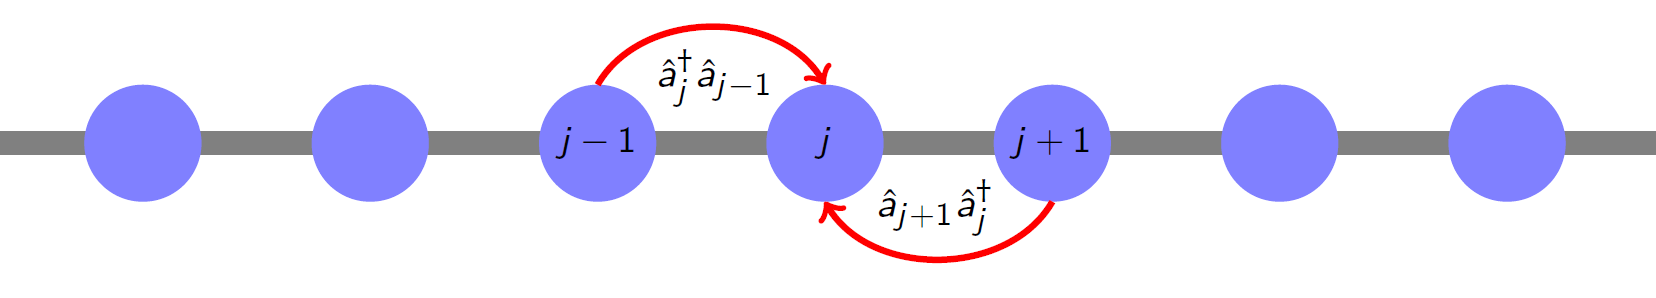
\includegraphics{lattice.png}
\caption{Hopping on a lattice}
\end{figure}

Fig. 1. Hopping on a 1D lattice. The operator \(\hat a_{j-1}\) deletes a
boson on site \(j-1\), and the operator \(\hat a_j^\dagger\) creates a
boson on site \(j\). The action of the operator
\(\hat a_j^\dagger \hat a_{j-1}\) therefore corrsponds to a boson
hopping to the right, and its adjoint represents a boson hopping to the
left. Figure made in TikZ.

    \hypertarget{mean-field-theory}{%
\subsubsection{Mean field theory}\label{mean-field-theory}}

    As mentioned previously, the main problem that arises in numerical
studies of the Bose-Hubbard model is the exponential scaling of the
Hilbert space with the number of lattice sites. The typical way to make
the problem more feasible for numerical simulations is to decouple the
lattice sites from one another, by employing a mean field theory.

To do this, we will look specifically at the operators in the
Hamiltonian that involve products of operators acting on different
lattice sites. These operators take the form
\(\hat a_{j}^\dagger \hat a_{k}\) where \(j,k\) correspond to indices of
neighbouring lattice sites. We can define a set of ``fluctuation
operators''

\begin{equation}
\delta \hat a_{j} \equiv \hat a_{j} - \psi_j
\end{equation}

where \(\psi_j \equiv \langle \hat a_{j} \rangle\) is the expectation
value of \(\hat a_j\) in the ground state. It follows that
\(\langle \delta \hat a_j \rangle \approx 0\) for states that are close
to the true ground state. We can then rewrite the products of operators
acting on different sites as:

\begin{align*}
\hat a_{j}^\dagger \hat a_{k} &= \Big( \delta \hat a_{j }^\dagger +\psi_j^* \Big)  \Big( \delta \hat a_{k } +\psi_k \Big)  \\
&= \delta \hat a_{j}^\dagger \delta \hat a_{k} +  \psi_j^*  \delta \hat a_{k } + \delta \hat a_{j}^\dagger \psi_k + \psi_{j}^* \psi_k . \\
\end{align*}

The mean field approximation is then to assume that correlations are
small enough that we can ignore the term which is second order in the
fluctuation operator. Under this assumption, the product becomes

\begin{align*} 
\hat a_{j}^\dagger \hat a_{k} &\approx \psi_j^*  \delta \hat a_{k } + \delta \hat a_{j}^\dagger \psi_k + \psi_{j}^* \psi_k \\
&=   \psi_j^*  \hat a_{k } +\hat a_{j}^\dagger \psi_k - \psi_{j}^* \psi_k 
\end{align*}

which is simply a sum of single site operators multiplied by a scalar
expectation value. Next, we will assume that the lattice is effectively
infinite in size, and is therefore translationally symmetric. Each
lattice site will therefore look the same, and we can assume that
\(\psi_0 = \psi_1 = \cdots = \psi_N \equiv \psi\). With the
aforementioned approximations, the Bose-Hubbard Hamiltonian becomes

\[H = -t \sum_j  \left[ \psi^* \hat a_j + \psi \hat a_j^\dagger - |\psi|^2 \right] + \frac U2 \sum_{j} \hat n_{j} \left( \hat n_{j} -1 \right) -\mu \sum_{j} \hat n_{j}\]

This choice of mean field approximation effectively decouples operators
acting on each site from one another, by replacing the operator with its
average value. By decoupling the sites from one another, the system of
interest will now scale linearly with the number of lattice sites,
rather than exponentially, and is thus manageable for efficient
numerical calculations.

The problem that remains is that we don't know the actual value of the
mean-field parameter \(\psi\). This can be obtained by assuming that the
system is in equilibrium, and so the actual valus of \(\psi\) will be
the one that minimizes the free energy of the system. Furthermore, we
are interested in the dynamics of this system at zero temperature, so
the free energy corresponds to the total internal energy.

    \hypertarget{probing-for-phase-transitions}{%
\subsubsection{Probing for phase
transitions}\label{probing-for-phase-transitions}}

    The final question that remains is how we will actually probe for phase
transitions in the model. Previous studies of this model have shown that
the ground state exists in two distinct phases, namely, a Mott-insulator
and a superfluid. It turns out that the expectation value
\(\psi = \langle a \rangle\) corresponds to the superfluid order
parameter, meaning that an insulating phase corresponds to \(\psi = 0\),
and a superfluid phase corresponds to \(\psi \neq 0\) {[}4{]}.

    \hypertarget{methods}{%
\subsection{Methods}\label{methods}}

    \hypertarget{exact-diagonalization}{%
\subsubsection{Exact diagonalization}\label{exact-diagonalization}}

    The first method that will be explored is the method of exact
diagonalization. We will start by explicitely constructing the
Hamiltonian matrix, by computing the matrix elements of the Hamiltonian
for a single site

\[\langle m | H | n \rangle = -t \psi^* \sqrt{n} \delta_{m,n-1} - t\psi \sqrt{n+1} \delta_{m,n+1} + \left(t |\psi|^2 + \frac{U}{2} n(n-1) - \mu n\right) \delta_{m,n}\]

for a given parameter set \((t,U,\mu)\). By dividing by the on-site
interaction energy \(U\), we make this Hamiltonian dimensionless, and
effectively reduce the problem to two free parameters
\(\left( \frac{t}{U},\frac{\mu}{U} \right)\). Some arbitrary state is
taken to be our initial guess, and the value of \(\psi\) is computed
accordingly. In principle, any number of bosons can occupy the lattice
site, however, we truncate the Hilbert space to \(N=10\) particles per
site, so the wavefunction takes the form

\[| \phi_0 \rangle = \sum_{x=0}^N \beta_x | x \rangle \]

for some \(\beta_0,\beta_1,\ldots,\beta_N\). The Hamiltonian matrix is
then numerically diagonalized, and the state \(| \phi_0 \rangle\) is
then updated to be the lowest energy eigenvector of this Hamiltonian.
The Hamiltonian matrix elements are then recomputed using the new state,
and the process is repeated until a self-consistent value of the order
parameter \(\psi\) is obtained. The phase of the ground state is then
inferred using the value of \(\psi\). The set of tools used for exact
diagonalization can be found in the appendix, or in the attached
exact\_diag.py module.

We will begin by analyzing how the energy behaves as a function of the
order parameter. What we expect is that the order parameter is zero in
the low-hopping limit \(t/U \ll 1\), corresponding to an insulating
phase, and at some critical hopping amplitude, there should be an
insulator-superfluid transition, where \(\psi\) becomes nonzero. The
following plot shows how the ground state energy depends on the value of
the order parameter, for varous choices in the hopping amplitude.

    \begin{Verbatim}[commandchars=\\\{\}]
{\color{incolor}In [{\color{incolor}3}]:} \PY{c+c1}{\PYZsh{}Import module I wrote for exact diagonalization calculations}
        \PY{k+kn}{import} \PY{n+nn}{exact\PYZus{}diag}
        
        \PY{c+c1}{\PYZsh{}Set system parameters}
        \PY{n}{mu} \PY{o}{=} \PY{l+m+mf}{0.5}
        \PY{n}{t} \PY{o}{=} \PY{p}{[}\PY{l+m+mf}{0.13}\PY{p}{,}\PY{l+m+mf}{0.17}\PY{p}{,}\PY{l+m+mf}{0.21}\PY{p}{]}
        
        \PY{c+c1}{\PYZsh{}Iterate through possible order parameters}
        \PY{n}{psi} \PY{o}{=} \PY{n}{np}\PY{o}{.}\PY{n}{linspace}\PY{p}{(}\PY{o}{\PYZhy{}}\PY{l+m+mf}{1.5}\PY{p}{,}\PY{l+m+mf}{1.5}\PY{p}{,}\PY{l+m+mi}{300}\PY{p}{)}
        
        \PY{c+c1}{\PYZsh{}Array to record energies}
        \PY{n}{E0} \PY{o}{=} \PY{n}{np}\PY{o}{.}\PY{n}{zeros}\PY{p}{(}\PY{p}{(}\PY{n+nb}{len}\PY{p}{(}\PY{n}{t}\PY{p}{)}\PY{p}{,}\PY{n+nb}{len}\PY{p}{(}\PY{n}{psi}\PY{p}{)}\PY{p}{)}\PY{p}{)}
        
        \PY{c+c1}{\PYZsh{}Create figure}
        \PY{n}{fig}\PY{p}{,} \PY{n}{ax} \PY{o}{=} \PY{n}{plt}\PY{o}{.}\PY{n}{subplots}\PY{p}{(}\PY{l+m+mi}{1}\PY{p}{,}\PY{n+nb}{len}\PY{p}{(}\PY{n}{t}\PY{p}{)}\PY{p}{,}\PY{n}{figsize}\PY{o}{=}\PY{p}{(}\PY{l+m+mi}{4}\PY{o}{*}\PY{n+nb}{len}\PY{p}{(}\PY{n}{t}\PY{p}{)}\PY{p}{,}\PY{l+m+mi}{4}\PY{p}{)}\PY{p}{,}\PY{n}{sharey} \PY{o}{=} \PY{k+kc}{True}\PY{p}{)}
        \PY{n}{ax}\PY{p}{[}\PY{l+m+mi}{0}\PY{p}{]}\PY{o}{.}\PY{n}{set\PYZus{}ylabel}\PY{p}{(}\PY{l+s+s1}{\PYZsq{}}\PY{l+s+s1}{\PYZdl{}E\PYZus{}0/U\PYZdl{}}\PY{l+s+s1}{\PYZsq{}}\PY{p}{,}\PY{n}{fontsize} \PY{o}{=} \PY{l+m+mi}{20}\PY{p}{)}
        
        \PY{k}{for} \PY{n}{j} \PY{o+ow}{in} \PY{n+nb}{range}\PY{p}{(}\PY{n+nb}{len}\PY{p}{(}\PY{n}{t}\PY{p}{)}\PY{p}{)}\PY{p}{:}
            
            \PY{k}{for} \PY{n}{k} \PY{o+ow}{in} \PY{n+nb}{range}\PY{p}{(}\PY{n+nb}{len}\PY{p}{(}\PY{n}{psi}\PY{p}{)}\PY{p}{)}\PY{p}{:}
                
                \PY{c+c1}{\PYZsh{}Compute ground state energy for given parameter set}
                \PY{n}{H} \PY{o}{=} \PY{n}{exact\PYZus{}diag}\PY{o}{.}\PY{n}{construct\PYZus{}hamiltonian}\PY{p}{(}\PY{n}{psi}\PY{p}{[}\PY{n}{k}\PY{p}{]}\PY{p}{,}\PY{n}{t}\PY{p}{[}\PY{n}{j}\PY{p}{]}\PY{p}{,}\PY{n}{mu}\PY{p}{)}
                \PY{n}{energy}\PY{p}{,} \PY{n}{state} \PY{o}{=} \PY{n}{exact\PYZus{}diag}\PY{o}{.}\PY{n}{groundstate}\PY{p}{(}\PY{n}{H}\PY{p}{)}
                
                \PY{c+c1}{\PYZsh{}Record energy}
                \PY{n}{E0}\PY{p}{[}\PY{n}{j}\PY{p}{]}\PY{p}{[}\PY{n}{k}\PY{p}{]} \PY{o}{=} \PY{n}{energy}
            
            \PY{c+c1}{\PYZsh{}Plot results}
            \PY{n}{ax}\PY{p}{[}\PY{n}{j}\PY{p}{]}\PY{o}{.}\PY{n}{plot}\PY{p}{(}\PY{n}{psi}\PY{p}{,}\PY{n}{E0}\PY{p}{[}\PY{n}{j}\PY{p}{]}\PY{p}{)}
            \PY{n}{ax}\PY{p}{[}\PY{n}{j}\PY{p}{]}\PY{o}{.}\PY{n}{set\PYZus{}xlim}\PY{p}{(}\PY{n}{np}\PY{o}{.}\PY{n}{min}\PY{p}{(}\PY{n}{psi}\PY{p}{)}\PY{p}{,}\PY{n}{np}\PY{o}{.}\PY{n}{max}\PY{p}{(}\PY{n}{psi}\PY{p}{)}\PY{p}{)}
            \PY{n}{ax}\PY{p}{[}\PY{n}{j}\PY{p}{]}\PY{o}{.}\PY{n}{set\PYZus{}xlabel}\PY{p}{(}\PY{l+s+s1}{\PYZsq{}}\PY{l+s+s1}{\PYZdl{}}\PY{l+s+s1}{\PYZbs{}}\PY{l+s+s1}{psi\PYZdl{}}\PY{l+s+s1}{\PYZsq{}}\PY{p}{,}\PY{n}{fontsize} \PY{o}{=} \PY{l+m+mi}{15}\PY{p}{)}
            \PY{n}{ax}\PY{p}{[}\PY{n}{j}\PY{p}{]}\PY{o}{.}\PY{n}{set\PYZus{}title}\PY{p}{(}\PY{l+s+s1}{\PYZsq{}}\PY{l+s+s1}{\PYZdl{}}\PY{l+s+s1}{\PYZbs{}}\PY{l+s+s1}{mu/U = \PYZdl{}}\PY{l+s+si}{\PYZob{}\PYZcb{}}\PY{l+s+s1}{, \PYZdl{}t/U = \PYZdl{}}\PY{l+s+si}{\PYZob{}\PYZcb{}}\PY{l+s+s1}{\PYZsq{}}\PY{o}{.}\PY{n}{format}\PY{p}{(}\PY{n}{mu}\PY{p}{,}\PY{n}{t}\PY{p}{[}\PY{n}{j}\PY{p}{]}\PY{p}{)}\PY{p}{,}\PY{n}{fontsize} \PY{o}{=} \PY{l+m+mi}{15}\PY{p}{)}
            \PY{n}{ax}\PY{p}{[}\PY{n}{j}\PY{p}{]}\PY{o}{.}\PY{n}{grid}\PY{p}{(}\PY{p}{)}
            
        \PY{n}{plt}\PY{o}{.}\PY{n}{show}\PY{p}{(}\PY{p}{)}
\end{Verbatim}


    \begin{center}
    \adjustimage{max size={0.9\linewidth}{0.9\paperheight}}{output_18_0.png}
    \end{center}
    { \hspace*{\fill} \\}
    
    As expected, the free energy, which in this zero-temperature system
corresponds to the ground state energy, is minimized by \(\psi = 0\) for
small values of the hopping amplitude. As the hopping amplitude
increases past some critical value, two distinct minima in the free
energy form, and so the ground state energy will correspond to a
non-zero value of the order parameter. Note that this diagram reveals a
symmetry in the Hamiltonian, as replacing \(\psi\) with \(-\psi\) leads
to the same ground state energy. This breaking of symmetry when the
ground state spontaneously chooses a value of \(\psi\) is indicative of
a continuous phase transition. To see this more clearly, we can look at
how the order parameter depends on the hopping amplitude directly.

    \begin{Verbatim}[commandchars=\\\{\}]
{\color{incolor}In [{\color{incolor}4}]:} \PY{c+c1}{\PYZsh{}Set system parameters}
        \PY{n}{mulist} \PY{o}{=} \PY{p}{[}\PY{l+m+mf}{0.5}\PY{p}{,}\PY{l+m+mf}{0.6}\PY{p}{,}\PY{l+m+mf}{0.7}\PY{p}{]}
        \PY{n}{tlist} \PY{o}{=} \PY{n}{np}\PY{o}{.}\PY{n}{linspace}\PY{p}{(}\PY{l+m+mf}{0.01}\PY{p}{,}\PY{l+m+mf}{0.25}\PY{p}{,}\PY{l+m+mi}{250}\PY{p}{)}
        
        \PY{c+c1}{\PYZsh{}Array to records values of psi}
        \PY{n}{psilist} \PY{o}{=} \PY{n}{np}\PY{o}{.}\PY{n}{zeros}\PY{p}{(}\PY{p}{(}\PY{n+nb}{len}\PY{p}{(}\PY{n}{tlist}\PY{p}{)}\PY{p}{)}\PY{p}{)}
        
        \PY{c+c1}{\PYZsh{}Create figure}
        \PY{n}{plt}\PY{o}{.}\PY{n}{figure}\PY{p}{(}\PY{n}{figsize}\PY{o}{=}\PY{p}{(}\PY{l+m+mi}{6}\PY{p}{,}\PY{l+m+mi}{5}\PY{p}{)}\PY{p}{)}
        
        \PY{c+c1}{\PYZsh{}Iterate through system parameters}
        \PY{k}{for} \PY{n}{j} \PY{o+ow}{in} \PY{n+nb}{range}\PY{p}{(}\PY{n+nb}{len}\PY{p}{(}\PY{n}{mulist}\PY{p}{)}\PY{p}{)}\PY{p}{:}
            \PY{k}{for} \PY{n}{k} \PY{o+ow}{in} \PY{n+nb}{range}\PY{p}{(}\PY{n+nb}{len}\PY{p}{(}\PY{n}{tlist}\PY{p}{)}\PY{p}{)}\PY{p}{:}
                
                \PY{c+c1}{\PYZsh{}Compute psi using exact diagonalization}
                \PY{n}{psilist}\PY{p}{[}\PY{n}{k}\PY{p}{]} \PY{o}{=} \PY{n}{exact\PYZus{}diag}\PY{o}{.}\PY{n}{find\PYZus{}psi}\PY{p}{(}\PY{n}{tlist}\PY{p}{[}\PY{n}{k}\PY{p}{]}\PY{p}{,}\PY{n}{mulist}\PY{p}{[}\PY{n}{j}\PY{p}{]}\PY{p}{)}
            
            \PY{c+c1}{\PYZsh{}Plot result}
            \PY{n}{plt}\PY{o}{.}\PY{n}{plot}\PY{p}{(}\PY{n}{tlist}\PY{p}{,}\PY{n}{psilist}\PY{p}{,}\PY{n}{label} \PY{o}{=}\PY{l+s+s1}{\PYZsq{}}\PY{l+s+s1}{\PYZdl{}}\PY{l+s+s1}{\PYZbs{}}\PY{l+s+s1}{mu/U= \PYZdl{}}\PY{l+s+si}{\PYZob{}\PYZcb{}}\PY{l+s+s1}{\PYZsq{}}\PY{o}{.}\PY{n}{format}\PY{p}{(}\PY{n}{mulist}\PY{p}{[}\PY{n}{j}\PY{p}{]}\PY{p}{)}\PY{p}{)}
        
        \PY{n}{plt}\PY{o}{.}\PY{n}{title}\PY{p}{(}\PY{l+s+s1}{\PYZsq{}}\PY{l+s+s1}{Superfluid Order Parameter}\PY{l+s+s1}{\PYZsq{}}\PY{p}{,}\PY{n}{fontsize} \PY{o}{=} \PY{l+m+mi}{18}\PY{p}{)}
        \PY{n}{plt}\PY{o}{.}\PY{n}{xlim}\PY{p}{(}\PY{n}{np}\PY{o}{.}\PY{n}{min}\PY{p}{(}\PY{n}{tlist}\PY{p}{)}\PY{p}{,}\PY{n}{np}\PY{o}{.}\PY{n}{max}\PY{p}{(}\PY{n}{tlist}\PY{p}{)}\PY{p}{)}
        \PY{n}{plt}\PY{o}{.}\PY{n}{xlabel}\PY{p}{(}\PY{l+s+s1}{\PYZsq{}}\PY{l+s+s1}{\PYZdl{}t/U\PYZdl{}}\PY{l+s+s1}{\PYZsq{}}\PY{p}{,}\PY{n}{fontsize} \PY{o}{=} \PY{l+m+mi}{20}\PY{p}{)}
        \PY{n}{plt}\PY{o}{.}\PY{n}{ylabel}\PY{p}{(}\PY{l+s+s1}{\PYZsq{}}\PY{l+s+s1}{\PYZdl{}}\PY{l+s+s1}{\PYZbs{}}\PY{l+s+s1}{psi\PYZdl{}}\PY{l+s+s1}{\PYZsq{}}\PY{p}{,}\PY{n}{fontsize} \PY{o}{=} \PY{l+m+mi}{25}\PY{p}{)}
        \PY{n}{plt}\PY{o}{.}\PY{n}{legend}\PY{p}{(}\PY{p}{)}
        \PY{n}{plt}\PY{o}{.}\PY{n}{grid}\PY{p}{(}\PY{p}{)}
        \PY{n}{plt}\PY{o}{.}\PY{n}{show}\PY{p}{(}\PY{p}{)}
\end{Verbatim}


    \begin{center}
    \adjustimage{max size={0.9\linewidth}{0.9\paperheight}}{output_20_0.png}
    \end{center}
    { \hspace*{\fill} \\}
    
    As expected, our results indicate that increasing the hopping amplitude
triggers a continuous phase transition, characterized by a kink in the
order parameter at a critical hopping amplitude. Finally, we can use
this exact diagonalization to compute a phase diagram of the
Bose-Hubbard model in the \(\mu-t\) parameter space. Since computing the
phase boundary requires many independent iterations through the
parameter space, this makes the task ideal for parallelization. I will
employ the multiprocessing Pool object to run the same number of tasks
that I have processors in parallel.

    \begin{Verbatim}[commandchars=\\\{\}]
{\color{incolor}In [{\color{incolor}5}]:} \PY{c+c1}{\PYZsh{}Count number of local CPUs}
        \PY{n}{NCPU} \PY{o}{=} \PY{n}{psutil}\PY{o}{.}\PY{n}{cpu\PYZus{}count}\PY{p}{(}\PY{p}{)} 
        
        \PY{c+c1}{\PYZsh{}Define list of chemical potentials to search over}
        \PY{n}{mulist} \PY{o}{=} \PY{n}{np}\PY{o}{.}\PY{n}{linspace}\PY{p}{(}\PY{l+m+mf}{0.001}\PY{p}{,}\PY{l+m+mf}{3.0}\PY{p}{,}\PY{l+m+mi}{250}\PY{p}{)}
        
        \PY{c+c1}{\PYZsh{}Need to include this if statement for some reason...}
        \PY{k}{if} \PY{n+nv+vm}{\PYZus{}\PYZus{}name\PYZus{}\PYZus{}} \PY{o}{==} \PY{l+s+s1}{\PYZsq{}}\PY{l+s+s1}{\PYZus{}\PYZus{}main\PYZus{}\PYZus{}}\PY{l+s+s1}{\PYZsq{}}\PY{p}{:}        
        
            \PY{k}{with} \PY{n}{Pool}\PY{p}{(}\PY{n}{NCPU}\PY{p}{)} \PY{k}{as} \PY{n}{p}\PY{p}{:}
                
                \PY{c+c1}{\PYZsh{}Compute boundary points using exact diagonalization}
                \PY{n}{bd} \PY{o}{=} \PY{n}{p}\PY{o}{.}\PY{n}{map}\PY{p}{(}\PY{n}{exact\PYZus{}diag}\PY{o}{.}\PY{n}{bd}\PY{p}{,} \PY{n}{mulist}\PY{p}{)}
\end{Verbatim}


    \begin{Verbatim}[commandchars=\\\{\}]
{\color{incolor}In [{\color{incolor}6}]:} \PY{n}{plt}\PY{o}{.}\PY{n}{figure}\PY{p}{(}\PY{n}{figsize}\PY{o}{=}\PY{p}{(}\PY{l+m+mi}{6}\PY{p}{,}\PY{l+m+mi}{6}\PY{p}{)}\PY{p}{)}
        \PY{n}{plt}\PY{o}{.}\PY{n}{plot}\PY{p}{(}\PY{n}{bd}\PY{p}{,}\PY{n}{mulist}\PY{p}{,}\PY{n}{color} \PY{o}{=} \PY{l+s+s1}{\PYZsq{}}\PY{l+s+s1}{black}\PY{l+s+s1}{\PYZsq{}}\PY{p}{)}
        \PY{n}{plt}\PY{o}{.}\PY{n}{title}\PY{p}{(}\PY{l+s+s1}{\PYZsq{}}\PY{l+s+s1}{Phases \PYZhy{} Exact Diagonalization}\PY{l+s+s1}{\PYZsq{}}\PY{p}{,}\PY{n}{fontsize} \PY{o}{=} \PY{l+m+mi}{20}\PY{p}{)}
        \PY{n}{plt}\PY{o}{.}\PY{n}{xlabel}\PY{p}{(}\PY{l+s+s1}{\PYZsq{}}\PY{l+s+s1}{\PYZdl{}t/U\PYZdl{}}\PY{l+s+s1}{\PYZsq{}}\PY{p}{,}\PY{n}{fontsize} \PY{o}{=} \PY{l+m+mi}{25}\PY{p}{)}
        \PY{n}{plt}\PY{o}{.}\PY{n}{ylabel}\PY{p}{(}\PY{l+s+s1}{\PYZsq{}}\PY{l+s+s1}{\PYZdl{}}\PY{l+s+s1}{\PYZbs{}}\PY{l+s+s1}{mu /U\PYZdl{}}\PY{l+s+s1}{\PYZsq{}}\PY{p}{,}\PY{n}{fontsize} \PY{o}{=} \PY{l+m+mi}{25}\PY{p}{)}
        \PY{n}{plt}\PY{o}{.}\PY{n}{xlim}\PY{p}{(}\PY{l+m+mi}{0}\PY{p}{,}\PY{l+m+mf}{0.2}\PY{p}{)}
        \PY{n}{plt}\PY{o}{.}\PY{n}{ylim}\PY{p}{(}\PY{n}{np}\PY{o}{.}\PY{n}{min}\PY{p}{(}\PY{n}{mulist}\PY{p}{)}\PY{p}{,}\PY{n}{np}\PY{o}{.}\PY{n}{max}\PY{p}{(}\PY{n}{mulist}\PY{p}{)}\PY{p}{)}
        
        \PY{n}{plt}\PY{o}{.}\PY{n}{text}\PY{p}{(}\PY{l+m+mf}{0.15}\PY{p}{,}\PY{l+m+mi}{3}\PY{o}{/}\PY{l+m+mi}{2}\PY{p}{,} \PY{l+s+s1}{\PYZsq{}}\PY{l+s+s1}{SF}\PY{l+s+s1}{\PYZsq{}}\PY{p}{,} \PY{n}{size}\PY{o}{=}\PY{l+m+mi}{24}\PY{p}{,} \PY{n}{ha}\PY{o}{=}\PY{l+s+s1}{\PYZsq{}}\PY{l+s+s1}{center}\PY{l+s+s1}{\PYZsq{}}\PY{p}{,} \PY{n}{va}\PY{o}{=}\PY{l+s+s1}{\PYZsq{}}\PY{l+s+s1}{center}\PY{l+s+s1}{\PYZsq{}}\PY{p}{)}
        \PY{k}{for} \PY{n}{n} \PY{o+ow}{in} \PY{n+nb}{range}\PY{p}{(}\PY{l+m+mi}{1}\PY{p}{,}\PY{l+m+mi}{4}\PY{p}{)}\PY{p}{:}
            \PY{n}{plt}\PY{o}{.}\PY{n}{text}\PY{p}{(}\PY{l+m+mf}{0.028}\PY{p}{,} \PY{n}{n}\PY{o}{\PYZhy{}}\PY{l+m+mf}{0.5}\PY{p}{,} \PY{l+s+s1}{\PYZsq{}}\PY{l+s+s1}{n = }\PY{l+s+si}{\PYZob{}\PYZcb{}}\PY{l+s+s1}{\PYZsq{}}\PY{o}{.}\PY{n}{format}\PY{p}{(}\PY{n}{n}\PY{p}{)}\PY{p}{,} \PY{n}{size}\PY{o}{=}\PY{l+m+mi}{20}\PY{p}{,} \PY{n}{ha}\PY{o}{=}\PY{l+s+s1}{\PYZsq{}}\PY{l+s+s1}{center}\PY{l+s+s1}{\PYZsq{}}\PY{p}{,} \PY{n}{va}\PY{o}{=}\PY{l+s+s1}{\PYZsq{}}\PY{l+s+s1}{center}\PY{l+s+s1}{\PYZsq{}}\PY{p}{)}
        
        \PY{n}{plt}\PY{o}{.}\PY{n}{show}\PY{p}{(}\PY{p}{)}
\end{Verbatim}


    \begin{center}
    \adjustimage{max size={0.9\linewidth}{0.9\paperheight}}{output_23_0.png}
    \end{center}
    { \hspace*{\fill} \\}
    
    As we see, a very peculiar phase diagram arises. For low \(t/U\), the
ground state corresponds to a so-called Mott-insulator, and each of the
``lobe'' like regions correspond to insulators with different on-site
densities, i.e.~1 particle per lattice site in the bottom lobe, 2
particles per site in the next one, and so on. For a large enough
hopping amplitude, there is a phase transition and the ground state
becomes a superfluid, characterized by a nonzero value of \(\psi\). It
is interesting how as the on-site density increases, the lobes become
shorter, so the system requires a lower hopping amplitude to transition
to a superfluid.

This phase diagram is consistent with previous studies of the
Bose-Hubbard model, such as Ref. {[}4{]}.

    \hypertarget{variational-principle}{%
\subsubsection{Variational principle}\label{variational-principle}}

    Next we will analyze the Bose-Hubbard phase diagram in the context of
the variational principle. The variational principle is an
extraordinarily powerful technique that relies on a simple fact: the
true ground state of a system is the one that minimizes the expectation
value of the Hamiltonian \(\langle \hat H \rangle\). The proof of this
is relatively straightforward. Consider some system whose time evolution
is governed by the Hamiltonian operator \(\hat H\). Let
\(E_0 \leq E_1 \leq E_2 \leq \cdots\) be the ordered list of energy
eigenvalues, and \(\{ | E_n \rangle \}\) the set of orthonormal energy
eigenstates. Any normalized wavefunction can then be expanded as a
superposition of energy eigenstates

\begin{equation*}
| \Psi(t) \rangle = \sum_n c_n e^{-i E_n t} | E_n \rangle
\end{equation*}

for some collection of complex numbers \(\{c_n\}\) such that \$\sum\_n
\textbar{}c\_n\textbar{}\^{}2 =1 \$. It then follows that

\begin{align*}
\langle \Psi | \hat H  |\Psi \rangle= \sum_{mn} c_m^* c_n \langle \phi_m | \hat H | \phi_n \rangle =\sum_{mn} c_m^* c_n E_n  \langle  \phi_m | \phi_n \rangle  = \sum_n |c_n|^2 E_n \geq  \sum_n |c_n|^2 E_0 = E_0
\end{align*}

where the inequality comes from the fact that \(E_n \geq E_0\) for all
\(n\). By minimizing the function \(\langle \hat H \rangle\) with
respect to all possible wavefunctions \$ \textbar{} \psi \rangle\$, we
are therefore guaranteed to obtain a ground state. In cases where the
ground state is degenerate, one can construct the eigenspace
corresponding to the eigenvalue \(E_0\) by repeating the minimization
procedure for different trial wavefunctions.

In the case of the Bose-Hubbard model, the mean field Hamiltonian for a
single site is given by

\begin{equation*}
\hat H = - t \left( \psi^* \hat a + \psi \hat a^\dagger - |\psi|^2 \right) + \frac{U}{2}  \hat n (\hat n-1) -\mu \hat n.
\end{equation*}

The expectation value is therefore given by

\begin{equation}
\langle \hat H \rangle = -t |\psi|^2 + \frac{U}{2} \langle \hat n (\hat n-1) \rangle - \mu \langle \hat n \rangle.
\end{equation}

We will use a trial wavefunction of the form

\begin{equation*}
| \phi_0 \rangle = \sum_{x=0}^N \beta_x | x \rangle
\end{equation*}

where we have truncated the Hilbert space, so that the maximum number of
bosons on a site is \(N=10\). We can assume that the expansion
coefficients of the trial wavefunction are real, as the Hamiltonian
matrix in the occupation number basis is real. It follows that

\begin{align*}
\psi  = \langle \phi_0 | \hat a | \phi_0 \rangle &= \sum_{x,y=0}^N  \beta_x \beta_y \langle x | \hat a | y \rangle \\
&= \sum_{x,y=0}^N \beta_x \beta_y \sqrt{y} \langle x | y-1 \rangle \\
&= \sum_{x,y=0}^N \beta_x \beta_y \sqrt{y} \delta_{x,y-1} \\
&=  \sum_{x=1}^{N} \beta_{x-1} \beta_{x} \sqrt{x}
\end{align*} and \begin{align*}
\langle \hat n \rangle &= \sum_{x,y=0}^N  \beta_x \beta_y \langle x | \hat n | y \rangle =  \sum_{x,y=0}^N  \beta_x \beta_y  y  \langle x | y \rangle = \sum_{x=1}^N \beta_x^2 x  \\
\langle \hat n (\hat n-1) \rangle &= \sum_{x,y=0}^N  \beta_x \beta_y \langle x| \hat n (\hat n-1) | y \rangle = \sum_{x=1}^N \beta_x^2 x(x-1).
\end{align*}

Plugging these into the expectation value, and dividing by
\(\langle \phi_0 | \phi_0 \rangle = \sum_{x=0}^N \beta_x^2\) to ensure
that the resulting wavefunction remains normalized, we get that

\begin{equation} 
\frac{ \langle \phi_0 | \hat H | \phi_0 \rangle}{\langle \phi_0 | \phi_0 \rangle} = \frac{1}{\sum_{x=0}^N \beta_x^2}\left[ -t \left( \sum_{x=1}^N \beta_{x-1}\beta_x \sqrt{x} \right)^2  + \sum_{x=0}^N \beta_x^2 \left( \frac{U}{2}x(x-1) -\mu x  \right)   \right].
\end{equation}

Then, by minimizing this expectation value with respect to the parameter
set \(\beta_0,...,\beta_N\), we obtain an estimate for the ground state.
Such a function is highly non-linear in the parameters \(\beta_j\), so
the quantity must be minimized numerically. The tools used to do this
can be found in the variational.py module, which employs the
scipy.optimize.minimize function to minimize the expectation value of
the Hamiltonian.

Using this method, a phase diagram is computed below.

    \begin{Verbatim}[commandchars=\\\{\}]
{\color{incolor}In [{\color{incolor}7}]:} \PY{c+c1}{\PYZsh{}Import module I wrote for variational calculations}
        \PY{k+kn}{import} \PY{n+nn}{variational}
        
        \PY{c+c1}{\PYZsh{}Count number of local CPUs}
        \PY{n}{NCPU} \PY{o}{=} \PY{n}{psutil}\PY{o}{.}\PY{n}{cpu\PYZus{}count}\PY{p}{(}\PY{p}{)}
        
        \PY{c+c1}{\PYZsh{}Define list of chemical potentials to search over}
        \PY{n}{mulist} \PY{o}{=} \PY{n}{np}\PY{o}{.}\PY{n}{linspace}\PY{p}{(}\PY{l+m+mf}{0.001}\PY{p}{,}\PY{l+m+mf}{3.0}\PY{p}{,}\PY{l+m+mi}{250}\PY{p}{)}
        
        \PY{c+c1}{\PYZsh{}Need to include this if statement for some reason...}
        \PY{k}{if} \PY{n+nv+vm}{\PYZus{}\PYZus{}name\PYZus{}\PYZus{}} \PY{o}{==} \PY{l+s+s1}{\PYZsq{}}\PY{l+s+s1}{\PYZus{}\PYZus{}main\PYZus{}\PYZus{}}\PY{l+s+s1}{\PYZsq{}}\PY{p}{:}        
        
            \PY{k}{with} \PY{n}{Pool}\PY{p}{(}\PY{n}{NCPU}\PY{p}{)} \PY{k}{as} \PY{n}{p}\PY{p}{:}
                
                \PY{c+c1}{\PYZsh{}Compute boundary points using exact diagonalization}
                \PY{n}{bd} \PY{o}{=} \PY{n}{p}\PY{o}{.}\PY{n}{map}\PY{p}{(}\PY{n}{variational}\PY{o}{.}\PY{n}{bd}\PY{p}{,} \PY{n}{mulist}\PY{p}{)}
\end{Verbatim}


    \begin{Verbatim}[commandchars=\\\{\}]
{\color{incolor}In [{\color{incolor}8}]:} \PY{n}{plt}\PY{o}{.}\PY{n}{figure}\PY{p}{(}\PY{n}{figsize}\PY{o}{=}\PY{p}{(}\PY{l+m+mi}{6}\PY{p}{,}\PY{l+m+mi}{6}\PY{p}{)}\PY{p}{)}
        \PY{n}{plt}\PY{o}{.}\PY{n}{plot}\PY{p}{(}\PY{n}{bd}\PY{p}{,}\PY{n}{mulist}\PY{p}{,}\PY{n}{color} \PY{o}{=} \PY{l+s+s1}{\PYZsq{}}\PY{l+s+s1}{black}\PY{l+s+s1}{\PYZsq{}}\PY{p}{)}
        \PY{n}{plt}\PY{o}{.}\PY{n}{title}\PY{p}{(}\PY{l+s+s1}{\PYZsq{}}\PY{l+s+s1}{Phases \PYZhy{} Variational methods}\PY{l+s+s1}{\PYZsq{}}\PY{p}{,}\PY{n}{fontsize} \PY{o}{=} \PY{l+m+mi}{20}\PY{p}{)}
        \PY{n}{plt}\PY{o}{.}\PY{n}{xlabel}\PY{p}{(}\PY{l+s+s1}{\PYZsq{}}\PY{l+s+s1}{\PYZdl{}t/U\PYZdl{}}\PY{l+s+s1}{\PYZsq{}}\PY{p}{,}\PY{n}{fontsize} \PY{o}{=} \PY{l+m+mi}{25}\PY{p}{)}
        \PY{n}{plt}\PY{o}{.}\PY{n}{ylabel}\PY{p}{(}\PY{l+s+s1}{\PYZsq{}}\PY{l+s+s1}{\PYZdl{}}\PY{l+s+s1}{\PYZbs{}}\PY{l+s+s1}{mu /U\PYZdl{}}\PY{l+s+s1}{\PYZsq{}}\PY{p}{,}\PY{n}{fontsize} \PY{o}{=} \PY{l+m+mi}{25}\PY{p}{)}
        \PY{n}{plt}\PY{o}{.}\PY{n}{xlim}\PY{p}{(}\PY{l+m+mi}{0}\PY{p}{,}\PY{l+m+mf}{0.2}\PY{p}{)}
        \PY{n}{plt}\PY{o}{.}\PY{n}{ylim}\PY{p}{(}\PY{n}{np}\PY{o}{.}\PY{n}{min}\PY{p}{(}\PY{n}{mulist}\PY{p}{)}\PY{p}{,}\PY{n}{np}\PY{o}{.}\PY{n}{max}\PY{p}{(}\PY{n}{mulist}\PY{p}{)}\PY{p}{)}
        
        \PY{n}{plt}\PY{o}{.}\PY{n}{text}\PY{p}{(}\PY{l+m+mf}{0.15}\PY{p}{,}\PY{l+m+mi}{3}\PY{o}{/}\PY{l+m+mi}{2}\PY{p}{,} \PY{l+s+s1}{\PYZsq{}}\PY{l+s+s1}{SF}\PY{l+s+s1}{\PYZsq{}}\PY{p}{,} \PY{n}{size}\PY{o}{=}\PY{l+m+mi}{24}\PY{p}{,} \PY{n}{ha}\PY{o}{=}\PY{l+s+s1}{\PYZsq{}}\PY{l+s+s1}{center}\PY{l+s+s1}{\PYZsq{}}\PY{p}{,} \PY{n}{va}\PY{o}{=}\PY{l+s+s1}{\PYZsq{}}\PY{l+s+s1}{center}\PY{l+s+s1}{\PYZsq{}}\PY{p}{)}
        \PY{k}{for} \PY{n}{n} \PY{o+ow}{in} \PY{n+nb}{range}\PY{p}{(}\PY{l+m+mi}{1}\PY{p}{,}\PY{l+m+mi}{4}\PY{p}{)}\PY{p}{:}
            \PY{n}{plt}\PY{o}{.}\PY{n}{text}\PY{p}{(}\PY{l+m+mf}{0.028}\PY{p}{,} \PY{n}{n}\PY{o}{\PYZhy{}}\PY{l+m+mf}{0.5}\PY{p}{,} \PY{l+s+s1}{\PYZsq{}}\PY{l+s+s1}{n = }\PY{l+s+si}{\PYZob{}\PYZcb{}}\PY{l+s+s1}{\PYZsq{}}\PY{o}{.}\PY{n}{format}\PY{p}{(}\PY{n}{n}\PY{p}{)}\PY{p}{,} \PY{n}{size}\PY{o}{=}\PY{l+m+mi}{20}\PY{p}{,} \PY{n}{ha}\PY{o}{=}\PY{l+s+s1}{\PYZsq{}}\PY{l+s+s1}{center}\PY{l+s+s1}{\PYZsq{}}\PY{p}{,} \PY{n}{va}\PY{o}{=}\PY{l+s+s1}{\PYZsq{}}\PY{l+s+s1}{center}\PY{l+s+s1}{\PYZsq{}}\PY{p}{)}
        
        \PY{n}{plt}\PY{o}{.}\PY{n}{show}\PY{p}{(}\PY{p}{)}
\end{Verbatim}


    \begin{center}
    \adjustimage{max size={0.9\linewidth}{0.9\paperheight}}{output_28_0.png}
    \end{center}
    { \hspace*{\fill} \\}
    
    As we see, the phase diagram generated with the variational method
exactly matches the result using exact diagonalization.

    \hypertarget{imaginary-time-propagation}{%
\subsubsection{Imaginary-time
propagation}\label{imaginary-time-propagation}}

    The final method that we will look it is known as imaginary-time
propagation. As this model is studied in the context of zero-temperature
bosons, the only states of interest will be the ones with the lowest
energy, known as the ground states. Rather than diagonalizing the entire
Hamiltonian operator, which would require constructing the entire
spectral decomposition, I use a method called \emph{imaginary time
propagation}, which allows one to independently compute the ground state
by solving the Schrödinger equation in a transformed time coordinate.
Such a method is often much more efficient than exact diagonalization,
especially when the Hamiltonian must be diagonalized numerically.

The general solution to the Schrödinger equation (in dimensionless
units)

\begin{equation*}
i \frac{\partial}{\partial t} | \psi(t) \rangle = \hat H | \psi(t) \rangle
\end{equation*}

for a time-independent Hamiltonian \(\hat H\) is given by some
superposition of stationary states

\begin{equation} \label{eqn:Eexpand}
| \psi(t) \rangle = \sum_{n=0}^\infty c_n e^{-i E_n t} | E_n \rangle
\end{equation}

where \(E_n\) and \(| E_n \rangle\) are the eigenvalues and eigenvectors
of the Hamiltonian operator respectively, and \(\{ c_n \}\) is some
collection of complex numbers {[}7{]}. Assume without loss of generality
that the energy eigenvalues are listed in increasing order, i.e.
\(E_0 \leq E_1 \leq E_2 \leq \cdots\). Defining the imaginary time
variable

\begin{equation} 
\tau \equiv i t,
\end{equation}

the expansion can be written as

\begin{equation*}
| \psi \left( -i \tau\right) \rangle = \sum_{n=0}^\infty c_n e^{- E_n \tau} | E_n \rangle = e^{- E_0 \tau}\left(c_0 | E_0 \rangle + \sum_{n=1}^\infty  c_n e^{- \left(E_n-E_0\right) \tau} | E_n \rangle \right).
\end{equation*}

Notice that as the imaginary time \(\tau\) gets large, the coefficients
of the higher energy states die off exponentially quickly, and we end up
with something proportional to the ground state

\begin{equation*}
| \psi \left( -i \tau \right) \rangle \propto | E_0 \rangle \qquad \text{as $\tau \to \infty$}.
\end{equation*}

Making the imaginary time substitution, to the Schrödinger equation, we
see that the propagation of the state \(|\psi \rangle\) in imaginary
time is governed by the differential equation
\begin{equation}\label{eqn:SchrodingerTau}
\frac{\partial}{\partial \tau} |\psi \rangle = -\hat H |\psi \rangle.
\end{equation}

Thus, by making some initial guess \(| \phi_0 \rangle\), we can obtain
the ground state by integrating the Schrödinger equation forward in
imaginary time. It is worth noting that the transformation to imaginary
time explicitly makes the Schrödinger equation non-unitary, and so the
ground state resulting from imaginary time propagation will need to be
explicitly re-normalized at each time step.

The tools used to implement the imaginary time propagation algorithm can
be found in the imag\_time.py module. To integrate the imaginary-time
Schrödinger equation, a 5th order Runge-Kutta routine is implemented,
and the wavefunction is explicitely re-normalized at each step in the
routine to make up for the exponentially decaying amplitudes.

    \begin{Verbatim}[commandchars=\\\{\}]
{\color{incolor}In [{\color{incolor}9}]:} \PY{c+c1}{\PYZsh{}Import module I wrote for imaginary time propagation}
        \PY{k+kn}{import} \PY{n+nn}{imag\PYZus{}time}
        
        \PY{c+c1}{\PYZsh{}Count number of local CPUs}
        \PY{n}{NCPU} \PY{o}{=} \PY{n}{psutil}\PY{o}{.}\PY{n}{cpu\PYZus{}count}\PY{p}{(}\PY{p}{)}
        
        \PY{c+c1}{\PYZsh{}Define list of chemical potentials to search over}
        \PY{n}{mulist} \PY{o}{=} \PY{n}{np}\PY{o}{.}\PY{n}{linspace}\PY{p}{(}\PY{l+m+mf}{0.001}\PY{p}{,}\PY{l+m+mf}{3.0}\PY{p}{,}\PY{l+m+mi}{100}\PY{p}{)}
        
        \PY{c+c1}{\PYZsh{}Need to include this if statement for some reason...}
        \PY{k}{if} \PY{n+nv+vm}{\PYZus{}\PYZus{}name\PYZus{}\PYZus{}} \PY{o}{==} \PY{l+s+s1}{\PYZsq{}}\PY{l+s+s1}{\PYZus{}\PYZus{}main\PYZus{}\PYZus{}}\PY{l+s+s1}{\PYZsq{}}\PY{p}{:}        
        
            \PY{k}{with} \PY{n}{Pool}\PY{p}{(}\PY{n}{NCPU}\PY{p}{)} \PY{k}{as} \PY{n}{p}\PY{p}{:}
                
                \PY{c+c1}{\PYZsh{}Compute boundary points using exact diagonalization}
                \PY{n}{bd} \PY{o}{=} \PY{n}{p}\PY{o}{.}\PY{n}{map}\PY{p}{(}\PY{n}{imag\PYZus{}time}\PY{o}{.}\PY{n}{bd}\PY{p}{,} \PY{n}{mulist}\PY{p}{)}
\end{Verbatim}


    \begin{Verbatim}[commandchars=\\\{\}]
{\color{incolor}In [{\color{incolor}10}]:} \PY{n}{plt}\PY{o}{.}\PY{n}{figure}\PY{p}{(}\PY{n}{figsize}\PY{o}{=}\PY{p}{(}\PY{l+m+mi}{6}\PY{p}{,}\PY{l+m+mi}{6}\PY{p}{)}\PY{p}{)}
         \PY{n}{plt}\PY{o}{.}\PY{n}{plot}\PY{p}{(}\PY{n}{bd}\PY{p}{,}\PY{n}{mulist}\PY{p}{,}\PY{n}{color} \PY{o}{=} \PY{l+s+s1}{\PYZsq{}}\PY{l+s+s1}{black}\PY{l+s+s1}{\PYZsq{}}\PY{p}{)}
         \PY{n}{plt}\PY{o}{.}\PY{n}{title}\PY{p}{(}\PY{l+s+s1}{\PYZsq{}}\PY{l+s+s1}{Phases \PYZhy{} Imaginary time propagation}\PY{l+s+s1}{\PYZsq{}}\PY{p}{,}\PY{n}{fontsize} \PY{o}{=} \PY{l+m+mi}{20}\PY{p}{)}
         \PY{n}{plt}\PY{o}{.}\PY{n}{xlabel}\PY{p}{(}\PY{l+s+s1}{\PYZsq{}}\PY{l+s+s1}{\PYZdl{}t/U\PYZdl{}}\PY{l+s+s1}{\PYZsq{}}\PY{p}{,}\PY{n}{fontsize} \PY{o}{=} \PY{l+m+mi}{25}\PY{p}{)}
         \PY{n}{plt}\PY{o}{.}\PY{n}{ylabel}\PY{p}{(}\PY{l+s+s1}{\PYZsq{}}\PY{l+s+s1}{\PYZdl{}}\PY{l+s+s1}{\PYZbs{}}\PY{l+s+s1}{mu /U\PYZdl{}}\PY{l+s+s1}{\PYZsq{}}\PY{p}{,}\PY{n}{fontsize} \PY{o}{=} \PY{l+m+mi}{25}\PY{p}{)}
         \PY{n}{plt}\PY{o}{.}\PY{n}{xlim}\PY{p}{(}\PY{l+m+mi}{0}\PY{p}{,}\PY{l+m+mf}{0.2}\PY{p}{)}
         \PY{n}{plt}\PY{o}{.}\PY{n}{ylim}\PY{p}{(}\PY{n}{np}\PY{o}{.}\PY{n}{min}\PY{p}{(}\PY{n}{mulist}\PY{p}{)}\PY{p}{,}\PY{n}{np}\PY{o}{.}\PY{n}{max}\PY{p}{(}\PY{n}{mulist}\PY{p}{)}\PY{p}{)}
         
         \PY{n}{plt}\PY{o}{.}\PY{n}{text}\PY{p}{(}\PY{l+m+mf}{0.15}\PY{p}{,}\PY{l+m+mi}{3}\PY{o}{/}\PY{l+m+mi}{2}\PY{p}{,} \PY{l+s+s1}{\PYZsq{}}\PY{l+s+s1}{SF}\PY{l+s+s1}{\PYZsq{}}\PY{p}{,} \PY{n}{size}\PY{o}{=}\PY{l+m+mi}{24}\PY{p}{,} \PY{n}{ha}\PY{o}{=}\PY{l+s+s1}{\PYZsq{}}\PY{l+s+s1}{center}\PY{l+s+s1}{\PYZsq{}}\PY{p}{,} \PY{n}{va}\PY{o}{=}\PY{l+s+s1}{\PYZsq{}}\PY{l+s+s1}{center}\PY{l+s+s1}{\PYZsq{}}\PY{p}{)}
         \PY{k}{for} \PY{n}{n} \PY{o+ow}{in} \PY{n+nb}{range}\PY{p}{(}\PY{l+m+mi}{1}\PY{p}{,}\PY{l+m+mi}{4}\PY{p}{)}\PY{p}{:}
             \PY{n}{plt}\PY{o}{.}\PY{n}{text}\PY{p}{(}\PY{l+m+mf}{0.028}\PY{p}{,} \PY{n}{n}\PY{o}{\PYZhy{}}\PY{l+m+mf}{0.5}\PY{p}{,} \PY{l+s+s1}{\PYZsq{}}\PY{l+s+s1}{n = }\PY{l+s+si}{\PYZob{}\PYZcb{}}\PY{l+s+s1}{\PYZsq{}}\PY{o}{.}\PY{n}{format}\PY{p}{(}\PY{n}{n}\PY{p}{)}\PY{p}{,} \PY{n}{size}\PY{o}{=}\PY{l+m+mi}{20}\PY{p}{,} \PY{n}{ha}\PY{o}{=}\PY{l+s+s1}{\PYZsq{}}\PY{l+s+s1}{center}\PY{l+s+s1}{\PYZsq{}}\PY{p}{,} \PY{n}{va}\PY{o}{=}\PY{l+s+s1}{\PYZsq{}}\PY{l+s+s1}{center}\PY{l+s+s1}{\PYZsq{}}\PY{p}{)}
         
         \PY{n}{plt}\PY{o}{.}\PY{n}{show}\PY{p}{(}\PY{p}{)}
\end{Verbatim}


    \begin{center}
    \adjustimage{max size={0.9\linewidth}{0.9\paperheight}}{output_33_0.png}
    \end{center}
    { \hspace*{\fill} \\}
    
    Once again, the phase diagram is consisten with both exact
diagonalization and variational approaches, as well as with the
literature studies of the Bose-Hubbard model. Note that for the
imaginary time propagation algorithm, I used a fewer number of data
points to compile the plot, since it was taking much longer than the
previous two algorithms.

    \hypertarget{algorithm-comparison}{%
\subsubsection{Algorithm comparison}\label{algorithm-comparison}}

    Given that each of the methods studied have been reliable for simulating
the Bose-Hubbard model, the real comparison of their performance comes
down to computational speed. To compare each of the algorithms, I will
record the time it takes to compute the phase boundary in the center of
the first insulator lobe \(\mu/U = 0.5\). Given that each of the use
precisely the same boundary search algorithm (i.e.~the one found in
bdsearch.py), this seems like a fair comparison.

    \begin{Verbatim}[commandchars=\\\{\}]
{\color{incolor}In [{\color{incolor}12}]:} \PY{o}{\PYZpc{}}\PY{k}{timeit} exact\PYZus{}diag.bd(0.5)
         \PY{o}{\PYZpc{}}\PY{k}{timeit} variational.bd(0.5)
         \PY{o}{\PYZpc{}}\PY{k}{timeit} imag\PYZus{}time.bd(0.5)
\end{Verbatim}


    \begin{Verbatim}[commandchars=\\\{\}]
4.57 s ± 37.2 ms per loop (mean ± std. dev. of 7 runs, 1 loop each)
903 ms ± 40.2 ms per loop (mean ± std. dev. of 7 runs, 1 loop each)
17.9 s ± 461 ms per loop (mean ± std. dev. of 7 runs, 1 loop each)

    \end{Verbatim}

    As we see, the variational method is an order of magnitude quicker than
the exact diagonalization method, and two orders of magnitude faster
than the imaginary time propagation algorithm. While the variational
method dominates in speed for this problem, the fact that we are
optimizing a highly non-linear function of many variables means that
this algorithm is most likely not very robust. As the size of either the
Hilbert space or the parameter space increases, I suspect that the
variational method would begin to fail, while the other two would remain
usable. While imaginary time propagation was the slowest algorithm
explored, it still remains a powerful tool in solving for the ground
state of systems in high-dimensional state spaces. For this problem, it
was simply overkill.

    \hypertarget{conclusion}{%
\subsubsection{Conclusion}\label{conclusion}}

    In this report, we looked at three distinct methods for simulating the
zero-temperature dynamics of the Bose-Hubbard model, an approximate
model for bosons in an optical lattice potential. Within the mean-field
approximation, each of these methods were able to reliably produce the
Bose-Hubbard phase diagram, by probing for a continuous phase
transition, and these diagrams were also consistent with previous
studies of this model. In terms of speed, we saw that the variational
method, implemented with the scipy.optimize library turned out to be the
most efficient algorithm for this specific model, however, I suspect
that this method would begin to fail in higher dimensional Hilbert
spaces, or in a higher dimensional parameter space.

With more time available, it would be interesting to see how imaginary
time propagation compares to the variational method in a more
complicated condensed matter system, such as the addition of nighbouring
interactions to the Bose-Hubbard model. Additionally, I am interested in
exploring this model outside of a mean-field theory, using methods such
as density matrix renormalization group.

    \hypertarget{bibliography}{%
\subsubsection{Bibliography}\label{bibliography}}

    {[}1{]} R. Landig, L. Hruby, N. Dogra, M. Landini, R. Mottl, T. Donner,
and T. Esslinger, Nature \textbf{532}, 476 (2016)

{[}2{]} G. Salomon, J. Koepsell, J. Vijayan, T. Hilker, J. Nespolo, L.
Pollet, I. Bloch, and C. Gross, Nature \textbf{565}, 56 (2018).

{[}3{]} S. Sachdev, \emph{Quantum Phase Transitions}, 2nd ed. (Cambridge
University Press, 2011).

{[}4{]} M. P. Fisher, P. B. Weichman, G. Grinstein, and D. S. Fisher,
Phys. Rev.~B \textbf{40}, 546 (1989).

{[}5{]} J. K. Freericks and H. Monien, Eur. Lett. \textbf{26}, 545
(1994).

{[}6{]} M. Greiner, O. Mandel, T. Esslinger, T. W. H¨ansch, and I.
Bloch, Nature \textbf{415}, 39 (2002).

{[}7{]} J. J. Sakurai, \emph{Modern Quantum Mechanics} (Addison-Wesley
Publishing, 1994).


    % Add a bibliography block to the postdoc
    
    
    
    \end{document}
